\documentclass[UTF8]{ctexart}

\title{电子技术基础实验最终实验报告}

\author{王磊\quad2022012972}

\date{\today}

\usepackage{geometry}
\geometry{a4paper,scale=0.8}

\usepackage{graphicx}
\usepackage{subfigure}
\usepackage{float}

\usepackage{amsmath}

\usepackage{listings}
\usepackage{xcolor}
\usepackage{framed}
\usepackage{placeins}
\usepackage{siunitx}
\lstdefinestyle{verilogStyle}{
    language=verilog,
    basicstyle=\ttfamily,
    keywordstyle=\color{blue},
    commentstyle=\color{green},
    stringstyle=\color{red},
    numbers=left,
    numberstyle=\tiny\color{gray},
    breaklines=true,
    showstringspaces=false,
    columns = fixed,
    basewidth = 0.5em,
    captionpos=b,
}
\newcommand{\subsubsubsection}[1]{\paragraph{#1}\mbox{}\\}
\setcounter{secnumdepth}{4} % how many sectioning levels to assign numbers to
\setcounter{tocdepth}{4} % how many sectioning levels to show in ToC
%设置段落间距
\setlength{\parskip}{0.5em}
%令小标题左对齐
\CTEXsetup[format={\Large\bfseries}]{section}
%首行不缩进
\setlength{\parindent}{0pt}
\begin{document}
\maketitle
\section{系统实现功能、架构和主要参数指标}
\subsection{实现功能}
最终构建的测量系统实现主要功能如图\ref{fig:system}所示。FPGA作为下位机,控制DAC实现双路数模转换,控制ADC实现双路模拟测量。使用simulink搭建上位机,通过串口与FPGA通信,实现数据的传输与显示。

\begin{figure}[!ht]
    \centering
    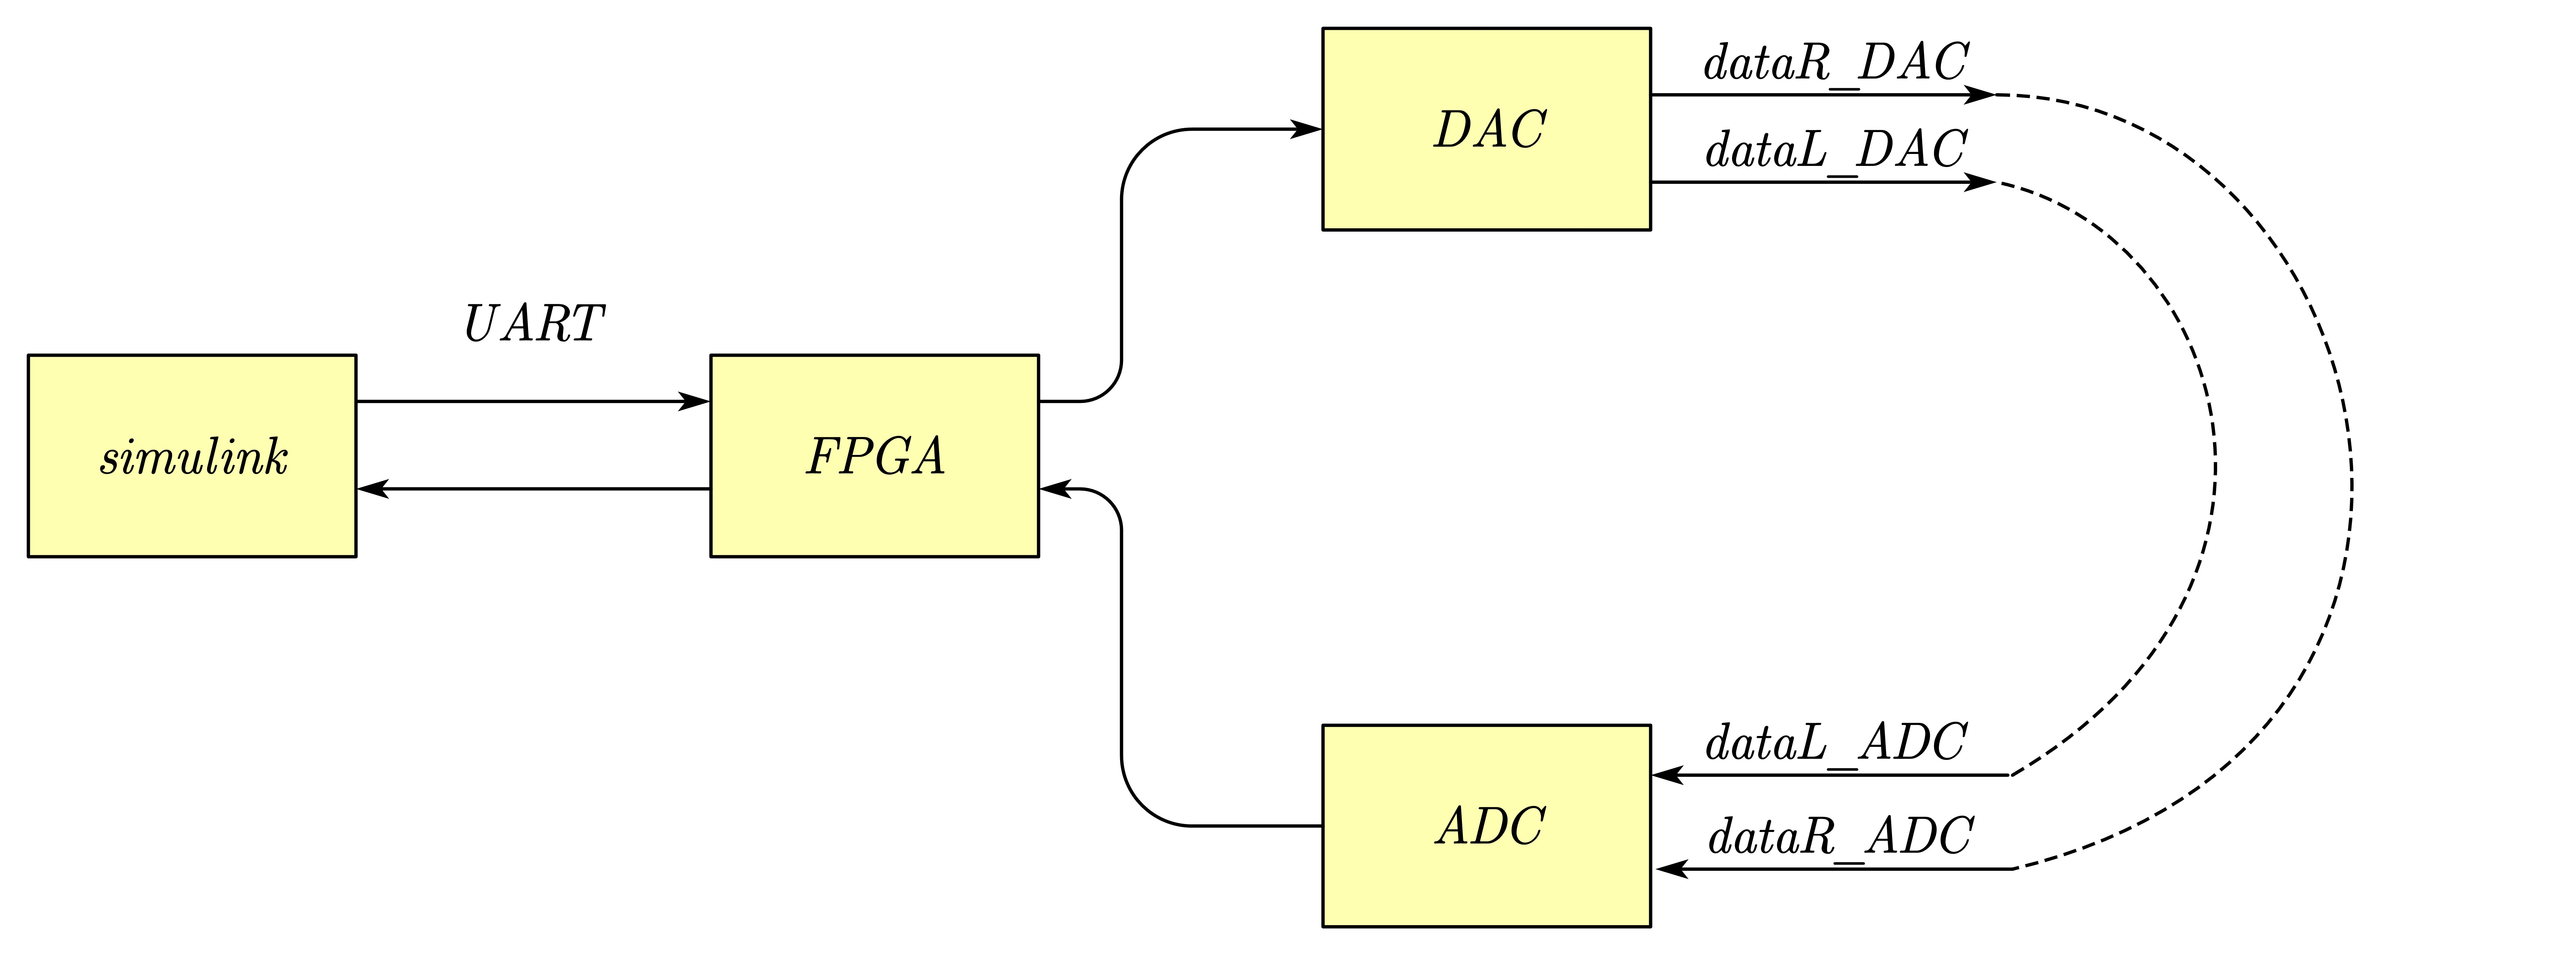
\includegraphics[width=0.8\textwidth]{system.png}
    \caption{测量系统功能图}
    \label{fig:system}
\end{figure}

\subsection{系统架构与参数指标}
实现系统功能的RTL电路图如图\ref{fig:rtl}所示。

\begin{figure}[!ht]
    \centering
    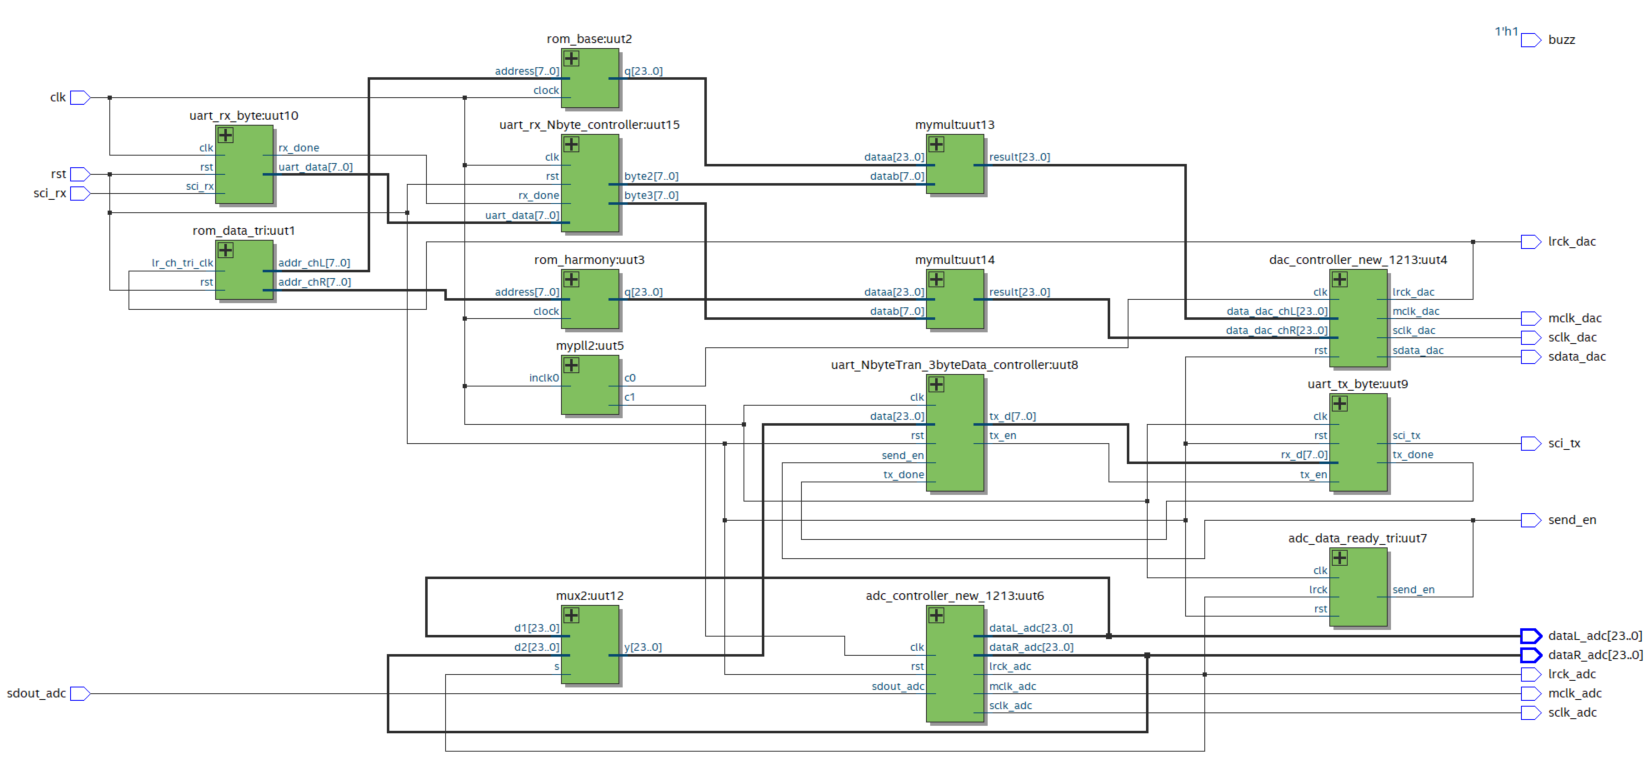
\includegraphics[width=0.8\textwidth]{rtl.png}
    \caption{系统RTL电路图}
    \label{fig:rtl}
\end{figure}

其中各模块实现的功能为:
\begin{itemize}
    \item \textbf{uart\_rx\_byte}:串口接收模块,以字节为单位接收上位机发送的数据。
    \item \textbf{uart\_rx\_Nbyte\_controller}:数据锁存模块,功能为锁存上位机发送的最近两个字节的数据,输送给乘法器。
    \item \textbf{rom\_data\_tri}:ROM触发模块,功能为根据DAC的lrck信号,更改输送给ROM模块的地址,实现数据的读取。
    \item \textbf{rom\_base\&harmony}:ROM模块,分别储存了基波和三位谐波的数据,根据rom\_data\_tri模块的地址,输出对应的数据。
    \item \textbf{mypll2}:锁相环模块,负责产生6.5535MHz的时钟信号,作为DAC的mclk信号;产生1.28MHz的时钟信号,作为ADC的mclk信号。
    \item \textbf{mymult}:乘法器模块,将上位机发送的数据与ROM模块输出的数据相乘,输出给DAC。
    \item \textbf{dac\_controller\_new\_1213}:DAC控制模块,负责控制DAC的工作模式,以及接收来自乘法器的数据,输出给DAC。
    \item \textbf{adc\_controlle\_new\_1213}:ADC控制模块,负责控制ADC的工作模式,以及接收来自ADC的数据,输出给MUX模块。
    \item \textbf{mux2}:MUX模块,根据ADC的lrck信号,选择输出ADC的左通道或右通道的数据。
    \item \textbf{adc\_data\_ready\_tri}:串口使能信号产生模块,根据ADC的lrck信号,使得当ADC采样后,给出串口使能信号,使得数据可以传输给上位机。
    \item \textbf{uart\_NbyteTran\_3byteData\_controller}:串口发送控制模块,负责将24位的数据分为3个字节,依此交给uart\_tx\_byte模块,实现数据发送,同时根据设定数据包的长度加入帧头和帧尾。
    \item \textbf{uart\_tx\_byte}:串口发送模块,以字节为单位,将数据发送给上位机。
\end{itemize}

系统的主要参数指标如表\ref{tab:parameter}所示。

\begin{table}[!ht]
    \centering
    \caption{系统主要参数指标}
    \label{tab:parameter}
    \begin{tabular}{|c|c|}
        \hline
        参数 & 指标 \\
        \hline
        DAC采样率 & 12800Hz \\
        \hline
        DAC量化精度 & 24bit \\
        \hline
        DAC通道数 & 2 \\
        \hline
        ADC采样率 & 5000Hz \\
        \hline
        ADC量化精度 & 24bit \\
        \hline
        ADC通道数 & 2 \\
        \hline
        通信协议 & UART \\
        \hline
        数据包长度 & 1000 \\
        \hline
    \end{tabular}
\end{table}

\FloatBarrier
\section{设计思路与具体实现}
除去老师提供的参考模块和由ip核自动生成的模块,由自己设计并实现的模块有:
\begin{itemize}
    \item rom\_data\_tri
    \item adc\_data\_ready\_tri
    \item mux2
\end{itemize}

下面分别介绍这三个模块的设计思路与具体实现。

\subsection{rom\_data\_tri}
该模块的代码如下:
\begin{framed}
    \begin{lstlisting}[style=verilogStyle]
module rom_data_tri (
    input lr_ch_tri_clk,
    input rst,
    output reg [7:0] addr_chL,
    output reg [7:0] addr_chR
);
    always @(posedge lr_ch_tri_clk or posedge rst) begin
        if (rst) begin
            addr_chL <= 8'd0;
        end else begin
            if (addr_chL == 8'd255) begin
                addr_chL <= 8'd0;
            end else begin
                addr_chL <= addr_chL + 1'b1;
            end
        end
    end

    always @(negedge lr_ch_tri_clk or posedge rst) begin
        if (rst) begin
            addr_chR <= 8'd0;
        end else begin
            if (addr_chR >= 8'd255) begin
                addr_chR <= 8'd0;
            end else begin
                addr_chR <= addr_chR + 1'b1;
            end
        end
    end

endmodule
    \end{lstlisting}
\end{framed}

该模块的功能是根据DAC的lrck信号,更改输送给ROM模块的地址,实现数据的读取。由于ROM模块的数据是以8位为单位读取的,因此需要两个地址,分别对应左通道和右通道。当lrck信号为上升沿时,左通道的地址加1;当lrck信号为下降沿时,右通道的地址加1。当地址达到255时,地址清零。

\subsection{adc\_data\_ready\_tri}
该模块的代码如下:
\begin{framed}
    \begin{lstlisting}[style=verilogStyle]
module adc_data_ready_tri(
    input clk,
    input rst,
    input lrck,
    output reg send_en
);

    reg pulse1, pulse2, pulse3;
    wire clk_edge;
    always @(posedge clk, posedge rst) begin
        if(rst) begin
            pulse1 <= 1'b0;
            pulse2 <= 1'b0;
            pulse3 <= 1'b0;
        end
        else begin
            pulse1 <= lrck;
            pulse2 <= pulse1;
            pulse3 <= pulse2;
        end
    end
    assign clk_edge = (pulse2 & ~pulse3) | (~pulse2 & pulse3);


    always @(posedge clk, posedge rst) begin
        if (rst) begin
            send_en <= 1'b0;
        end
        else begin
            if(clk_edge) begin
                send_en <= 1'b1;
            end
            else begin
                send_en <= 1'b0;
            end
        end
    end


endmodule
    \end{lstlisting}
\end{framed}

该模块的功能是根据ADC的lrck信号,使得当ADC采样后,给出串口使能信号,使得数据可以传输给上位机。当lrck信号发生跳变时,说明ADC进行了一次采样,打慢两拍以确保数据做好传输准备,给出一个脉冲信号,通知串口模块发送新的数据。

\subsection{mux2}
该模块的代码如下:
\begin{framed}
    \begin{lstlisting}[style=verilogStyle]
module mux2(
    input  s,
    input [23:0] d1,
    input [23:0] d2,
    output reg [23:0] y
);

    always @ (s or d1 or d2)
        case (s)
            1'd1: y <= d1;
            1'd0: y <= d2;
            default: y <= 24'd0;
        endcase

        endmodule

    \end{lstlisting}    
\end{framed}

该模块的功能是根据输入的s信号,选择输出d1或d2。当s为0时,输出d1;当s为1时,输出d2;其他情况输出0。其中ADC的lrck信号作为s信号输入,根据lrck信号的跳变,选择输出左通道或右通道的数据。

\FloatBarrier
\section{系统创新}
在实现本系统时,我并未采用老师提供的参考思路,即通过修改\textbf{uart\_NbyteTran\_3byteData\_controller}中的状态机实现两路数据的同时发送。

通过阅读ADC芯片的datasheet我了解到,ADC对哪个通道采样是通过lrck信号决定的,当lrck为1时,采样左通道;当lrck为0时,采样右通道。因此,我设计了mux2模块,根据lrck信号,选择输出左通道或右通道的数据。在实现单路数据发送时,我检测了lrck的上升沿作为数据发送的时机,因此只需要增加一行代码使得下降沿也成为数据发送的时机,就可以实现两路数据的同时发送。

\FloatBarrier
\section{存在问题与改进方向}
目前系统存在最大的问题在数据发送时由于没有更改状态机,因此每个数据包中左通道在前还是右通道在前是随机的,取决于重置后ADC的采样方式,存在一定概率出现左右通道数据错位的情况。解决这个问题的方法是在\textbf{uart\_NbyteTran\_3byteData\_controller}中增加一个或多个状态,根据lrck信号的跳变,判断当前采样的是左通道还是右通道,从而确定数据包中左右通道数据的顺序。
\end{document}